\section{About the Authors}\label{about-the-authors}

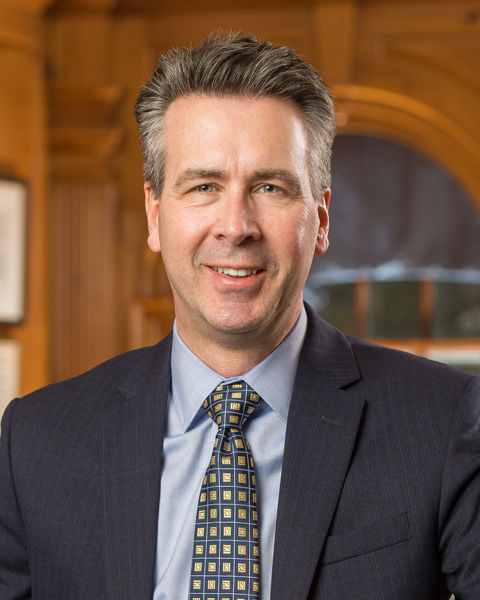
\includegraphics[width=1in]{./Fig/Ford.jpg}Ralph
Dr. Ralph Ford is chancellor of Penn State Erie, The Behrend College. As Penn State Behrend’s chief 
academic and administrative officer, he is responsible for all teaching, research, and outreach 
programs and activities of the college as well as overall campus operations.

Dr. Ford has more than 25 years of leadership experience in higher education and industry. He
 joined Penn State Behrend in 1994 as a faculty member in electrical and computer engineering, 
 subsequently serving as department chair.

In 2005, Dr. Ford was named director of the college’s School of Engineering. Under his leadership,
the school increased its national visibility as reflected in its rankings as one of the top 50 
undergraduate engineering programs in the country by U.S. News \& World Report.

In 2013, Dr. Ford assumed additional duties as associate dean for industry and external 
relations for the college. In this role, he led Penn State Behrend’s open-laboratory model
 of industry-academic collaboration, which matches students and faculty members with 
 private-sector partners for experiential student learning, applied research, and advanced
  product development. He also led the strategic partnership with Knowledge Park, the 
  college’s 100-acre technology park.

Prior to joining Penn State Behrend, Dr. Ford held engineering positions at IBM Microelectronics 
and Brookhaven National Laboratory. He is a past vice president and past member of the
 board of directors of the Institute of Electrical and Electronics Engineers, the largest technical 
 professional society in the world. Dr. Ford was a Fulbright Scholar at the Brno University of 
 Technology in 2005.

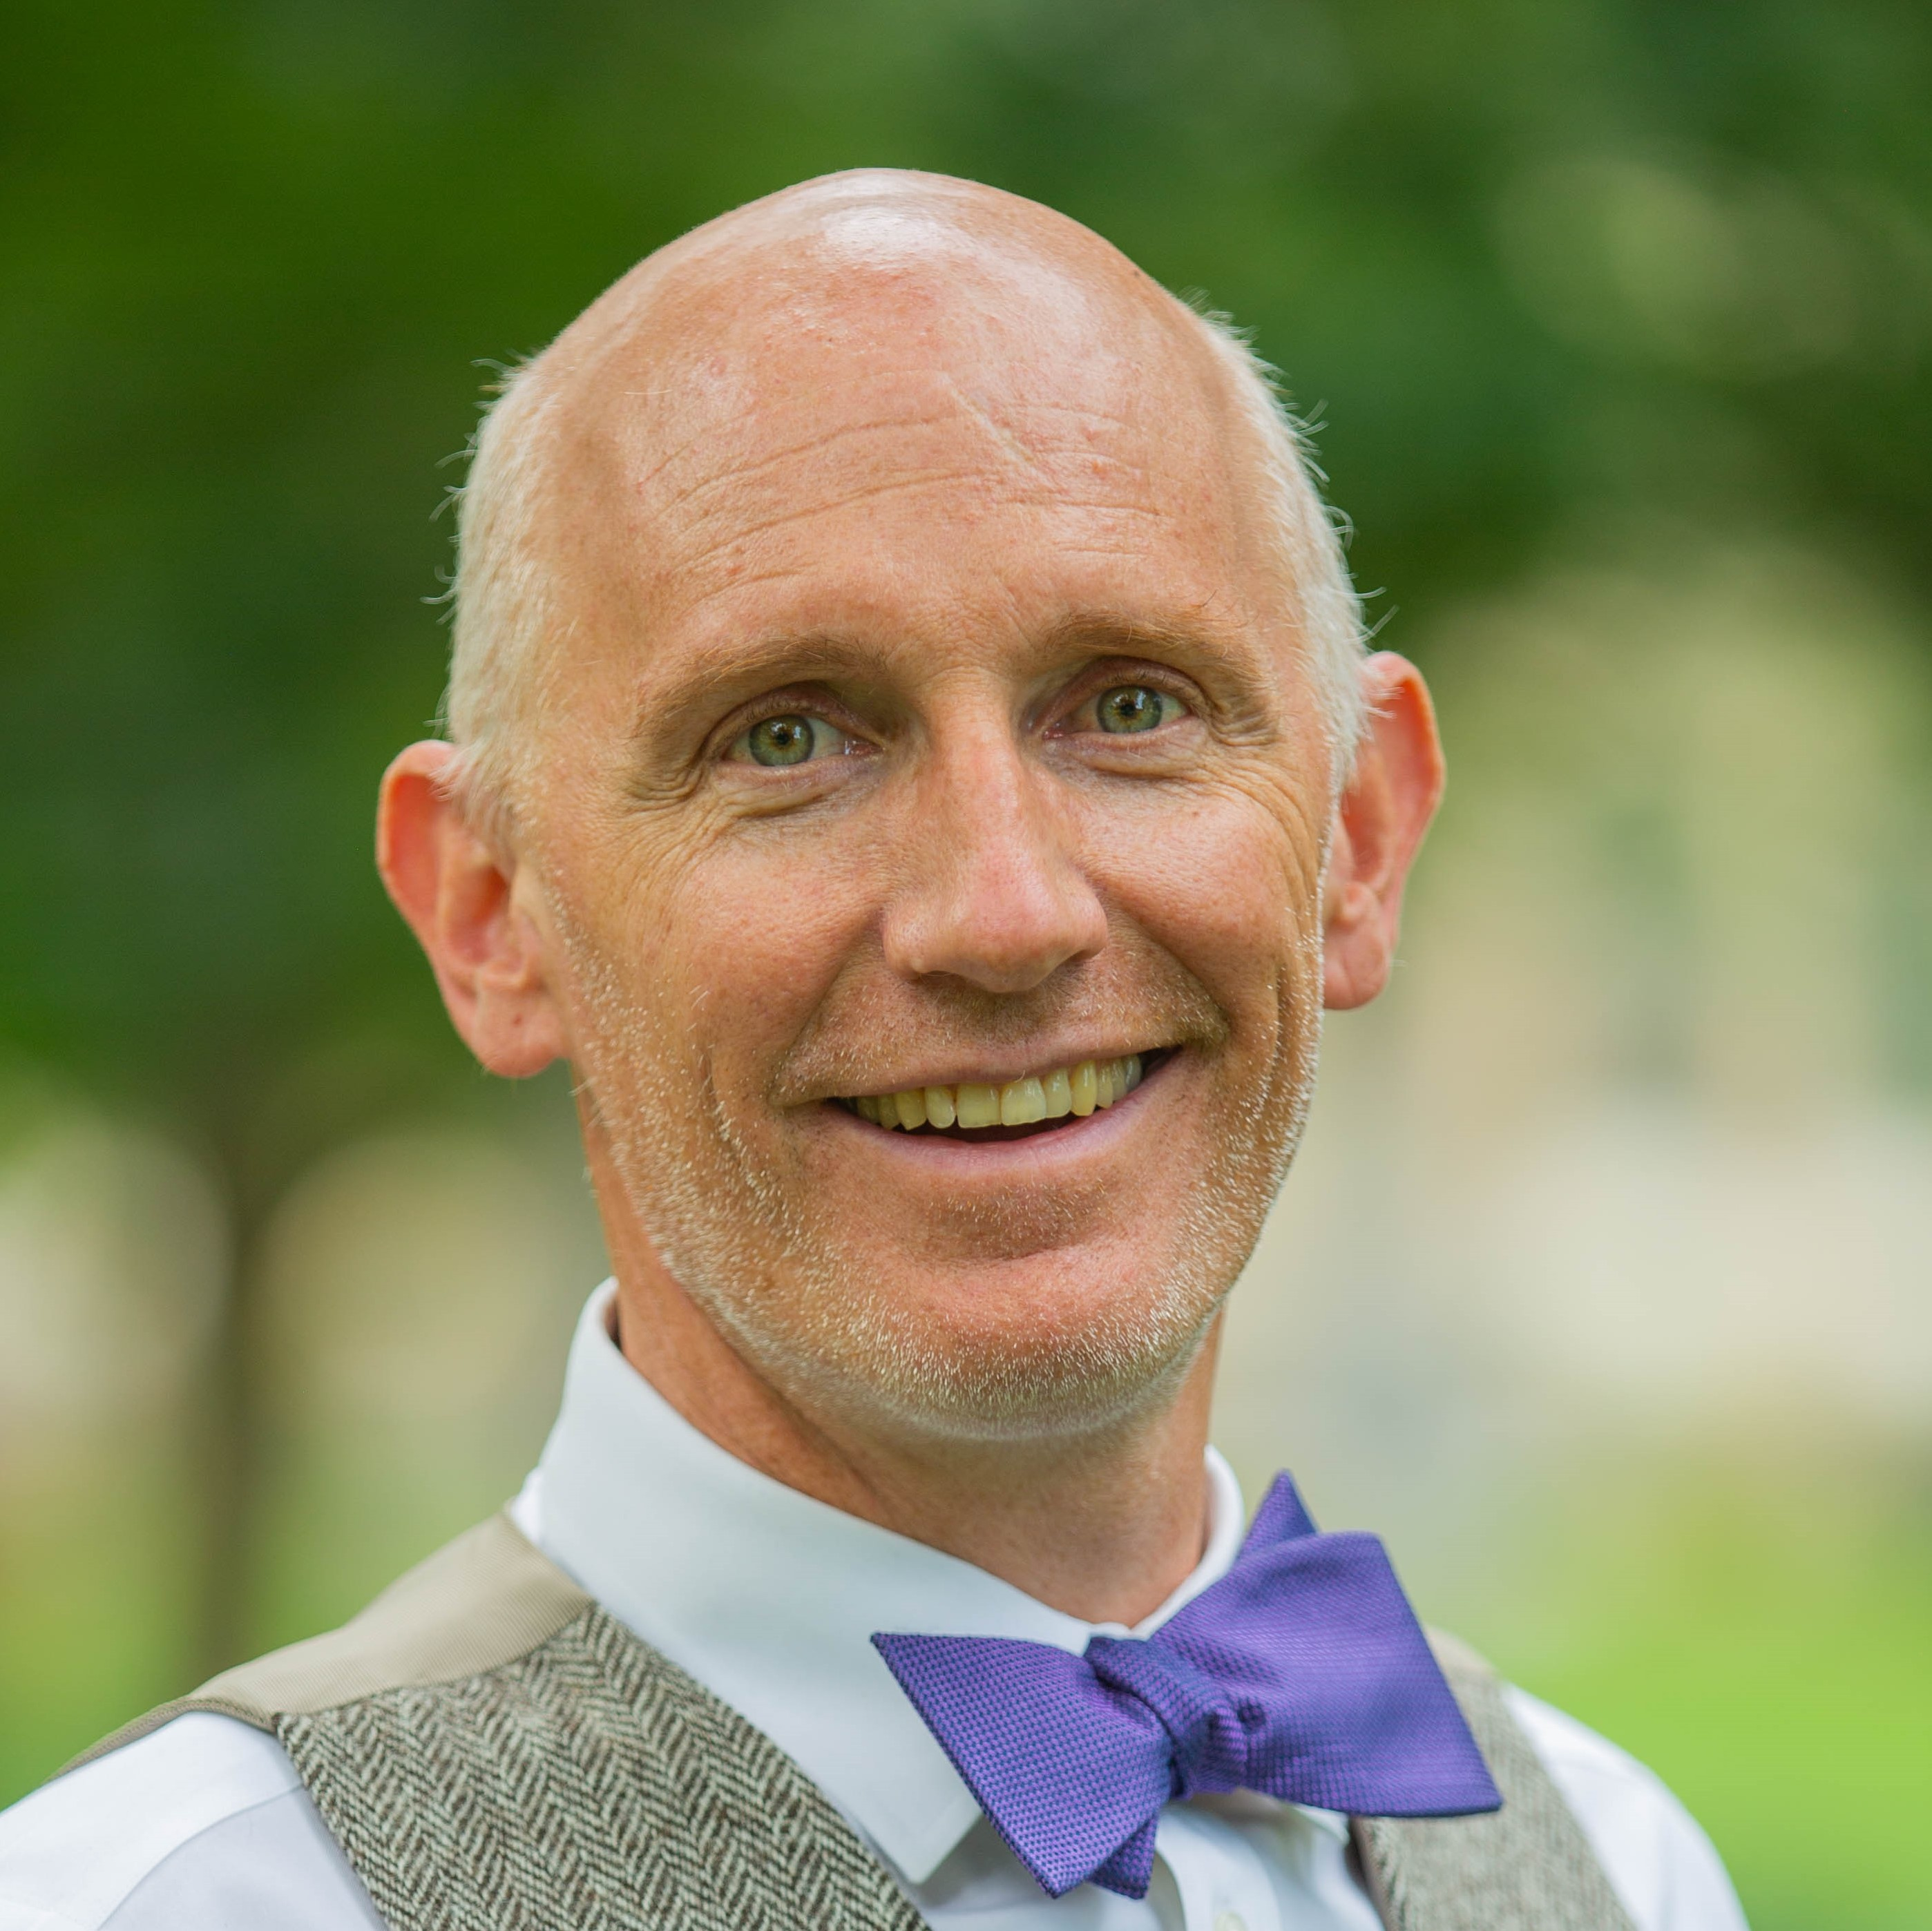
\includegraphics[width=1in]{./Fig/Coulston.jpg}Chris
Coulston obtained his Ph.D. in Computer Science and Engineering from the
Pennsylvania State University in 1999. He obtained his M.S. and B.S in
Computer Engineering from the Pennsylvania State University in 1994 and
1992 respectively. Chris has industry experience working for IBM in
Manassas, VA and Accu-Weather in State College, PA. He joined the
faculty at Penn State Erie, The Behrend College in 1999.  He served as 
served as Chairperson of Electrical and Computer Engineering program
for 9 yeears.  He is now a teaching professor at the Colorado School of Mines.
